\documentclass[tikz,border=10pt]{standalone}
\usetikzlibrary{calc}

\begin{document}
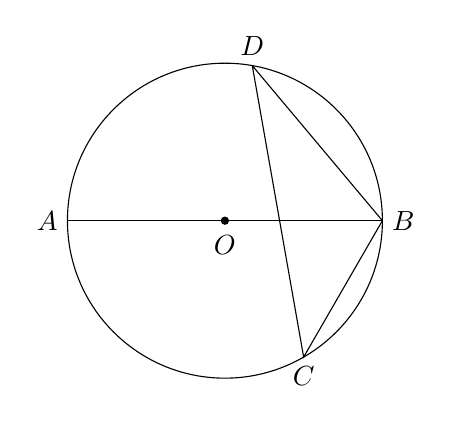
\begin{tikzpicture}
    % 1. 定义参数
    \def\r{2} % 圆的半径
    
    % 2. 绘制圆形
    \draw (0,0) circle (\r);
    
    % 3. 定义关键点坐标
    \coordinate (O) at (0,0);
    \coordinate (A) at (-\r,0);
    \coordinate (B) at (\r,0);
    % 使用极坐标确定 D 和 C 的位置
    \coordinate (D) at (80:\r);
    \coordinate (C) at (-60:\r);
    
    % 4. 绘制线段
    \draw (A) -- (B);       % 直径 AB
    \draw (D) -- (B) -- (C) -- (D); % 连接三角形/四边形边界
    
    % 5. 标记关键点
    \fill (O) circle (1.5pt) node[below=2pt] {$O$};
    \node[left] at (A) {$A$};
    \node[right] at (B) {$B$};
    \node[above] at (D) {$D$};
    \node[below] at (C) {$C$};
    
\end{tikzpicture}
\end{document}